\documentclass[12pt]{article}
\usepackage[utf8]{inputenc} % Obsługa kodowania utf8
\usepackage[T1]{fontenc} % Obsługa polskich znaków w fontach
\usepackage{graphicx} % Required for inserting images
\usepackage{float} 
\usepackage{geometry}
\usepackage{ragged2e}
\usepackage{listings}
\usepackage{xcolor}
\usepackage{caption} 
\usepackage{hyperref}

\captionsetup[figure]{name=Rys.}

% Ustawienia dla kolorów
\definecolor{codegreen}{rgb}{0,0.6,0}
\definecolor{codegray}{rgb}{0.5,0.5,0.5}
\definecolor{codepurple}{rgb}{0.58,0,0.82}
\definecolor{backcolour}{rgb}{1.0,1.0,1.0}

% Ustawienia dla wyglądu kodu
\lstdefinestyle{mystyle}{
    backgroundcolor=\color{backcolour},   
    commentstyle=\color{codegreen},
    keywordstyle=\color{blue},
    numberstyle=\tiny\color{codegray},
    stringstyle=\color{codepurple},
    basicstyle=\footnotesize,
    breakatwhitespace=false,         
    breaklines=true,                 
    captionpos=b,                    
    keepspaces=true,                 
    numbers=left,                    
    numbersep=5pt,                  
    showspaces=false,                
    showstringspaces=false,
    showtabs=false,                  
    tabsize=2
}

\lstset{style=mystyle}


\geometry{
    top=2cm,
    bottom=2cm,
    left=1cm,
    right=1cm
}


\graphicspath{{images/}}
\title{Projekt \par Bezzałogowe Obiekty Autonomiczne  \par \vspace{10pt} \textbf{Symulacja robota Unitree Go2 w środowisku ISSAC SIM}}
\date{}  




\begin{document}
\begin{figure}[t]
\centering
    
\includegraphics[width=0.8\textwidth]{Zdjęcia/Polsl.png}
\end{figure}

\maketitle
\vspace{150pt}
Skład sekcji: Filip Bazarnicki, Darian Bonk, Jakub Ligenza, Kacper Wach

Rok akademicki: 2024/25


Kierunek: Automatyka i Robotyka

Specjalizacja: Robotyka

Semestr: 1


\newpage

\section{Cel projektu}


Celem projektu była instalacja środowiska ISSAC SIM oraz jego odpowiednia konfiguracja, przygotowanie cyfrowego bliźniaka robota Unitree Go2, przeprowadzenie przykładowych symulacji w ISAAC SIM oraz nawiązanie połączenia między nim, a środowiskiem ROS2.

\section{Wstęp teoretyczny}
\subsection{Czym jest środowisko ISAAC SIM}

NVIDIA Isaac Sim to zaawansowane środowisko symulacyjne oparte na silniku Omniverse, stworzone z myślą o rozwoju i testowaniu algorytmów dla robotyki. Umożliwia realistyczną symulację fizyki, czujników oraz środowisk 3D, co pozwala na szybkie prototypowanie i walidację systemów autonomicznych bez konieczności fizycznego dostępu do sprzętu.
Symulator ten wspiera modelowanie robotów zgodne z formatem URDF (Unified Robot Description Format) oraz pozwala na integrację z popularnymi bibliotekami takimi jak ROS/ROS2, PyTorch, czy Isaac SDK. Dzięki realistycznemu odwzorowaniu działania sensorów (np. kamer RGB-D, LiDAR, IMU), możliwe jest testowanie algorytmów percepcji, lokalizacji, mapowania, planowania ruchu czy sterowania w warunkach zbliżonych do rzeczywistych.
Środowisko to odgrywa kluczową rolę w symulacji „cyfrowych bliźniaków” robotów, co znacząco obniża koszty i ryzyko związane z rzeczywistymi testami.

\subsection{Czym jest środowisko ROS2}

ROS 2 (Robot Operating System 2) to otwartoźródłowy system operacyjny dla robotów nowej generacji, zaprojektowany jako następca klasycznego ROS 1. Stanowi zaawansowaną platformę programistyczną do tworzenia, testowania i wdrażania oprogramowania dla systemów robotycznych, umożliwiając modularne projektowanie aplikacji z wykorzystaniem tzw. węzłów (nodes), które komunikują się ze sobą poprzez tematy (topics), usługi (services) oraz akcje (actions).


Jedną z kluczowych zmian w ROS 2 względem poprzednika jest zastosowanie standardu DDS (Data Distribution Service) jako warstwy komunikacyjnej, co zapewnia deterministyczne i wydajne przesyłanie danych między węzłami – również w sieciach rozproszonych.

ROS 2 współpracuje z popularnymi narzędziami robotycznymi i symulatorami (np. Gazebo, Isaac Sim, MoveIt 2), wspiera wiele języków programowania (C++, Python) i znajduje zastosowanie w robotyce przemysłowej, mobilnej, medycznej i badawczej.

\subsection{Czym jest robot Unitree Go2}

Unitree GO2 to zaawansowany, autonomiczny czteronożny robot mobilny (quadruped robot) opracowany przez firmę Unitree Robotics. Został zaprojektowany z myślą o wszechstronnych zastosowaniach w dziedzinach takich jak badania naukowe, eksploracja terenów trudnodostępnych, edukacja, patrolowanie oraz rozwój algorytmów sztucznej inteligencji i percepcji środowiska.
Robot GO2 jest sterowany za pomocą systemu ROS 2, co umożliwia integrację z istniejącymi narzędziami i frameworkami robotycznymi. Dzięki zastosowaniu silników o wysokim momencie obrotowym i zaawansowanym algorytmom stabilizacji, GO2 potrafi poruszać się stabilnie w zmiennych warunkach terenowych.


\section{Instalacja i konfiguracja środowiska ISSAC SIM oraz ROS2}

W projekcie korzystaliśmy z systemu Ubuntu 22.04, wykorzystaliśmy system Linux ze względu na potrzebę wykorzystania środowiska ROS2 w projekcie, co jest prostsze w systemach linuxowych.   

\subsection{Instalacja środowiska ISAAC SIM}

Ponieważ nie da się już pobrać ISAAC SIM bezpośrednio przy użyciu Omniverse Launcher, pobraliśmy ręcznie archiwum ze strony NVIDIA:

\begin{itemize}
    \item Strona: https://developer.nvidia.com/isaac-sim
    \item Wersja: Isaac Sim 4.5.0
\end{itemize}

Po pobraniu rozpakowaliśmy plik i możliwe było już uruchomienie środowiska ISAAC SIM. Można to zrobić, wchodząc do katalogu, w którym umieszczone zostały rozpakowane pliki i wpisując ./isaac-sim.sh lub alternatywnie isaac-sim.selector.sh.

 

\subsection{Instalacja środowiska ROS2}

Źródłem wykonanej instalacji była oficjalna dokumentacja ROS 2 dla wersji Humble (Ubuntu Development Setup):

 https://docs.ros.org/en/humble/Installation/Alternatives/Ubuntu-Development-Setup.html


\subsubsection{Krok 1: Konfiguracja lokalizacji UTF-8}
Na początku upewniliśmy się, że system ma skonfigurowane środowisko lokalizacyjne obsługujące UTF-8.


\texttt{sudo locale-gen en\_US en\_US.UTF-8}

\texttt{sudo update-locale LC\_ALL=en\_US.UTF-8 LANG=en\_US.UTF-8}

\texttt{export LANG=en\_US.UTF-8}

Sprawdziliśmy, czy ustawienia lokalne są prawidłowe:

\texttt{locale}

\subsubsection{Krok 2: Instalacja zależności systemowych}
Zainstalowaliśmy wymagane pakiety narzędziowe i kompilacyjne:

\texttt{sudo apt update \&\& sudo apt install -y}


\texttt{build-essential cmake git wget curl}


\texttt{gnupg lsb-release python3-colcon-common-extensions}


\texttt{python3-pip python3-vcstool python3-rosdep}
\\

Zainicjowaliśmy narzędzie rosdep:

\texttt{sudo rosdep init}


\texttt{rosdep update}


\subsubsection{Krok 3: Utworzenie przestrzeni roboczej i pobranie kodu ROS 2}

Stworzyliśmy katalog roboczy i pobraliśmy plik repozytoriów:


\texttt{mkdir -p $\sim$/ros2\_humble/src}

\texttt{cd $\sim$/ros2\_humble}

\texttt{wget https://raw.githubusercontent.com/ros2/ros2/humble/ros2.repos}

\texttt{vcs import src < ros2.repos}

\subsubsection{Krok 4: Instalacja zależności pakietów ROS 2}

Zainstalowaliśmy wszystkie zależności wymagane do kompilacji (pomijając rti-connext, którego nie potrzebujemy).


\texttt{rosdep install --from-paths src --ignore-src -r -y}

\texttt{--skip-keys "fastcdr rti-connext-dds-6.0.1 urdfdom\_headers}


\subsubsection{Krok 5: Kompilacja ROS 2}

Rozpoczęliśmy kompilację całego środowiska z wykorzystaniem colcon:

\texttt{cd $\sim$/ros2\_humble}

\texttt{colcon build --symlink-install}

Ten proces trwał kilkanaście minut.


\subsubsection{Krok 6: Konfiguracja środowiska}

Po zakończeniu kompilacji dodaliśmy ROS 2 do zmiennych środowiskowych:

\texttt{echo "source $\sim$/ros2\_humble/install/setup.bash" $>>$ $\sim$/.bashrc}

\texttt{source $\sim$/.bashrc}

Dzięki temu komenda ros2 była dostępna z każdego terminala.

\subsubsection{Weryfikacja działania ros2 }

Przeprowadziliśmy podstawowy test komunikacji między dwoma węzłami:

Terminal 1:

\texttt{ros2 run demo\_nodes\_cpp talker}


Terminal 2:

\texttt{ros2 run demo\_nodes\_cpp listener}
\\
Terminal listener poprawnie odbierał wiadomości wysyłane przez talker, co potwierdziło, że środowisko działa.

\newpage
\section{Cyfrowy bliźniak robota Unitree Go2}

W środowisku ISSAC SIM znajduje się gotowy model cyfrowego bliźniaka robota Unitree Go2, w celu umieszczenia go na scenie otwartego programu należy odnaleźć go w oknie Isaac Sim Assets i dodać go, wciskając przycisk Load as Reference lub przeciągając jego ikonę na scenę. Widok okna Isaac Sim Assets przedstawiony jest na rysunku \ref{fig:Assets}. Widok umieszczonego w symulacji robota przedstawiony jest na rysunku \ref{fig:cyfrowyBlizniak}. Na rysunku \ref{fig:groundPlane} pokazane jest, jak dodać podłogę w scenie, należy wybrać w górnym pasku Create, następnie Physics,  a na końcu wcisnąć Ground Plane.  

\begin{figure}[h]
    \centering
    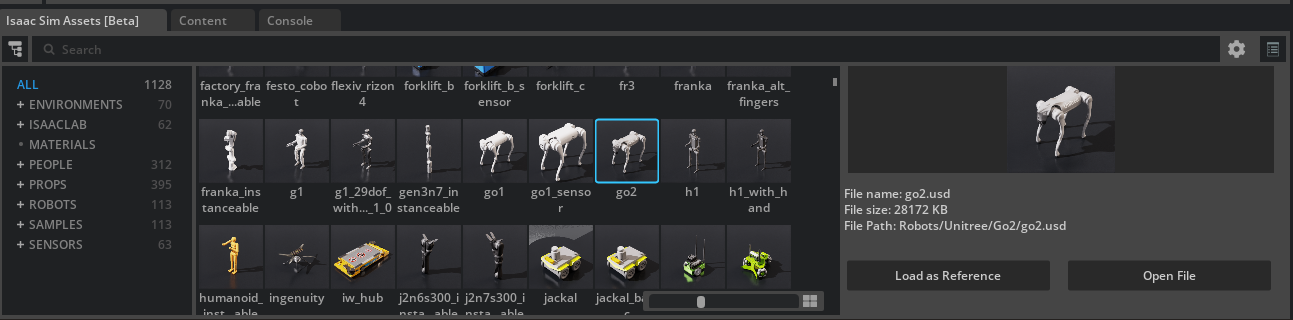
\includegraphics[width=0.75\linewidth]{Zdjęcia/bibliotekaAssets.png}
    \caption{Biblioteka dostępnych robotów Isaac Sim Assets.}
    \label{fig:Assets}
\end{figure}

\clearpage

\begin{figure}[h]
    \centering
    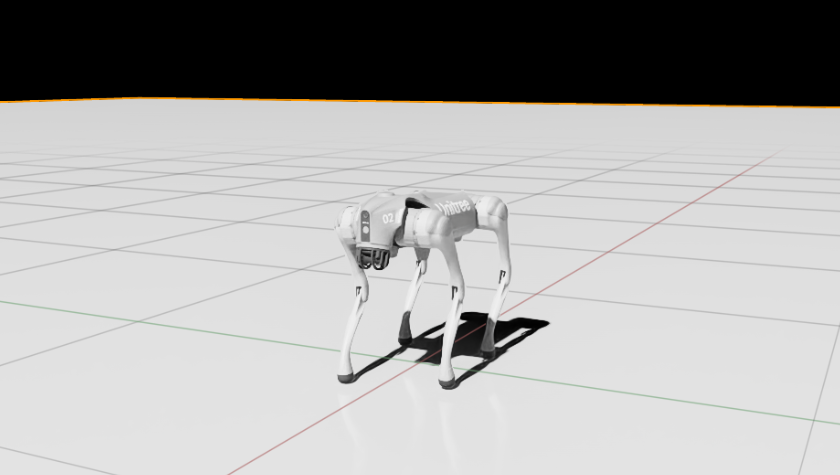
\includegraphics[width=0.7\linewidth]{Zdjęcia/cyfrowyBlizniakUnitryGo2.png}
    \caption{Cyfrowy bliźniak robota Unitree Go2 w środowisku ISAAC SIM.}
    \label{fig:cyfrowyBlizniak}
\end{figure}

\begin{figure}[h]
    \centering
    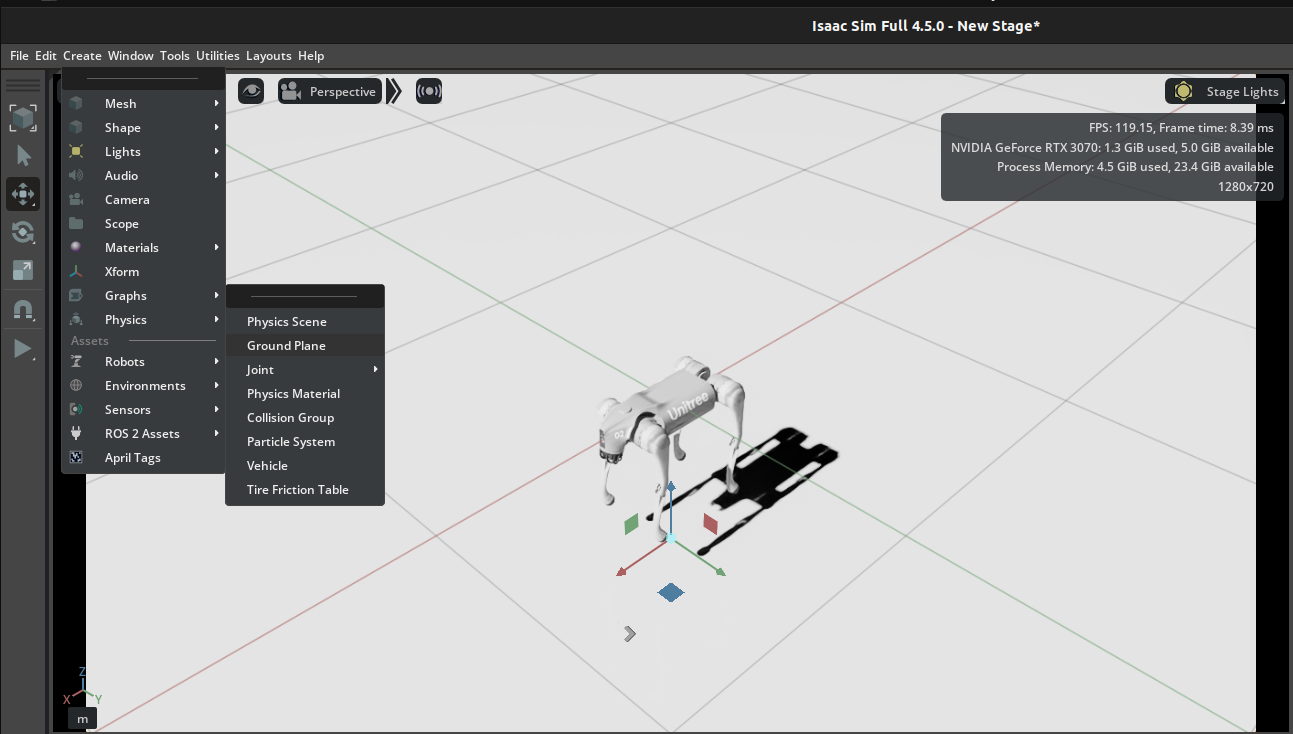
\includegraphics[width=0.7\linewidth]{Zdjęcia/groundPlane.png}
    \caption{Dodanie podłoża w ISSAC SIM.}
    \label{fig:groundPlane}
\end{figure}

\clearpage

\section{Sterowania robotem przy pomocy środowiska ROS2}

Wszystkie potrzebne pliki źródłowe do sterowania sterowania robotem znajdują się w linku poniżej.

https://drive.google.com/drive/folders/1fdtBgbXUCxln3wdQgWUAGIBdBf-2Qv9z
\vspace{10pt}

Żeby możliwe było sterowanie robotem Unitree Go2 przy pomocy środowiska ROS2, wymagane jest dodanie do projektu specjalnego grafu z instrukcjami w formie bloków (Action Graph).Na rysunku \ref{fig:jakDodacAction} pokazane jest jak dodać Action Graph, a rysunku \ref{fig:actionGraph} widoczne są potrzebne do sterowania robotem bloki oraz połączenia między nimi. 

\begin{figure}[h]
    \centering
    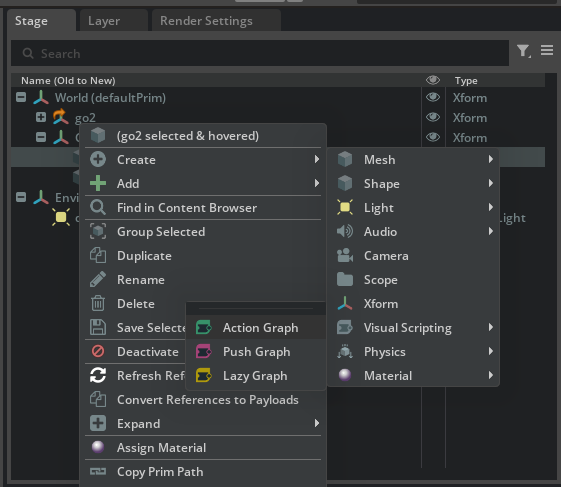
\includegraphics[width=0.5\linewidth]{Zdjęcia/dodanieActionGraph.png}
    \caption{Dodanie Action Graph do cyfrowego bliźniaka Unitree Go2}
    \label{fig:jakDodacAction}
\end{figure}

\clearpage

\begin{figure}[h]
    \centering
    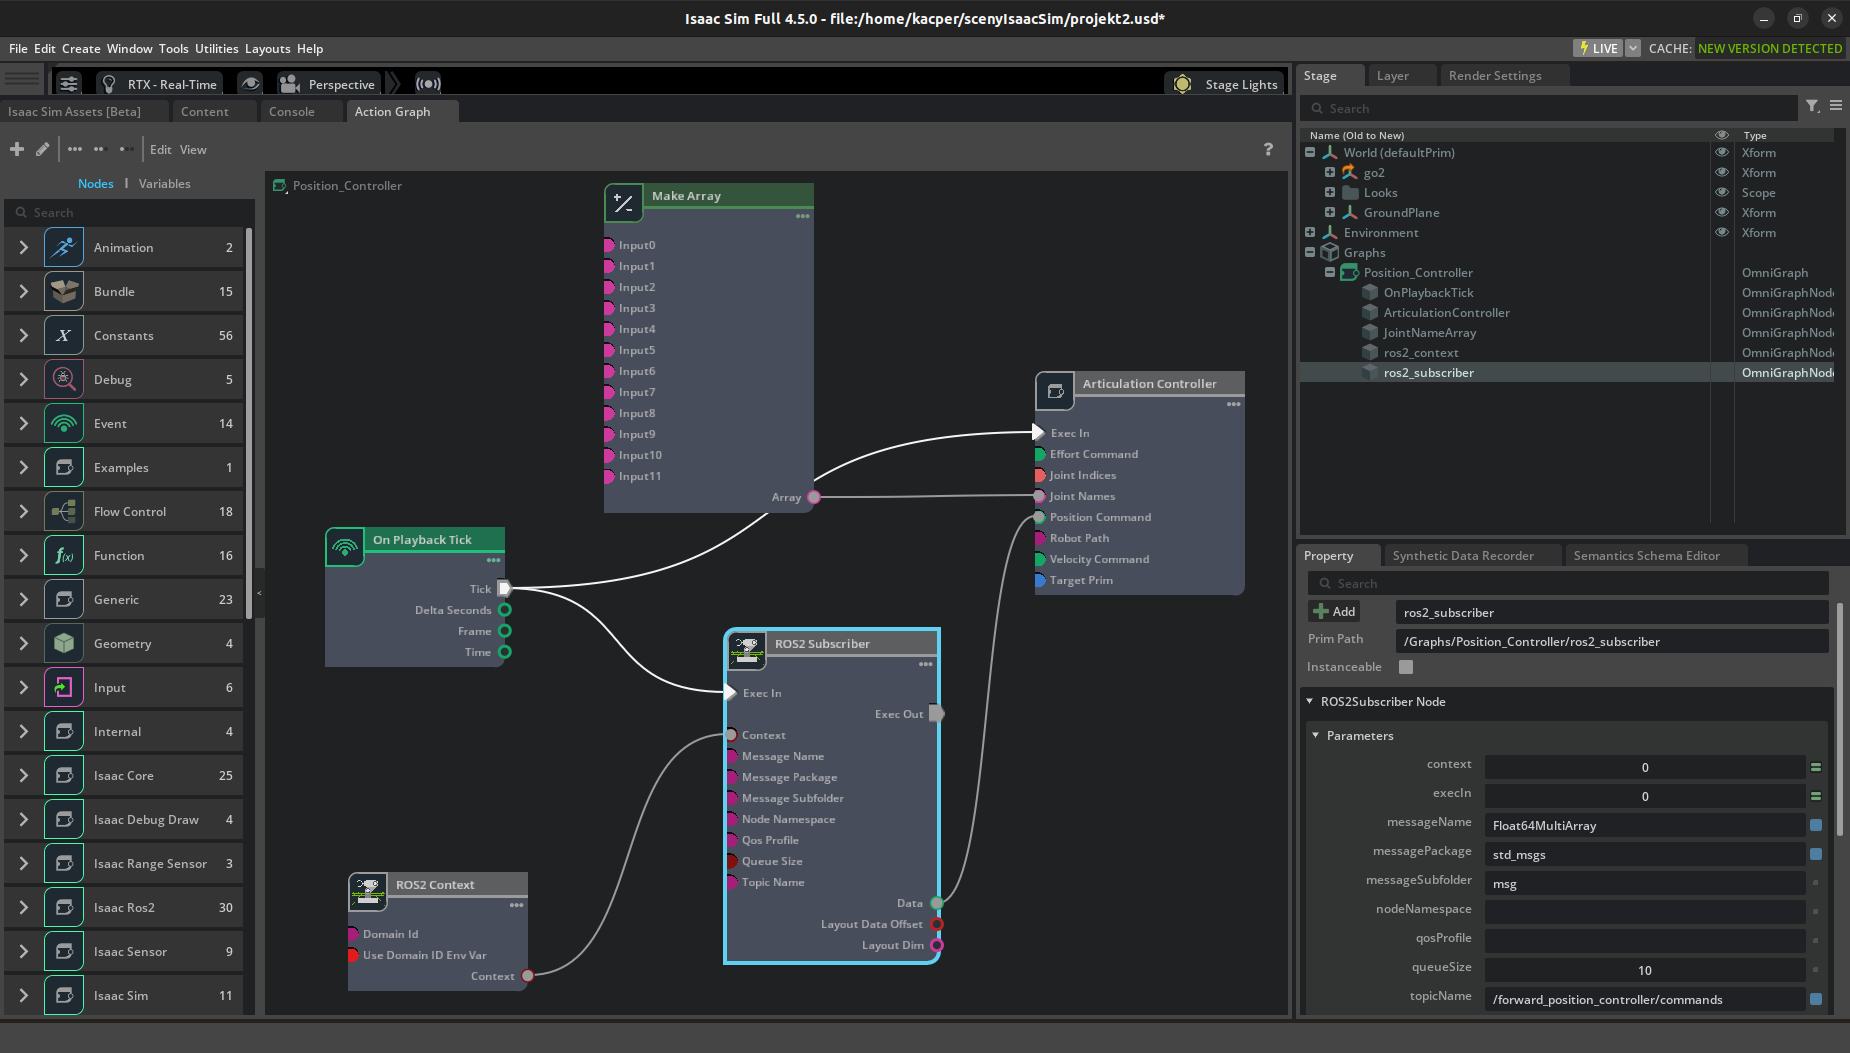
\includegraphics[width=0.75\linewidth]{Zdjęcia/actionGraph.png}
    \caption{Action Graph do nawiązania komunikacji między ROS2 oraz ISAAC SIM.}
    \label{fig:actionGraph}
\end{figure}


Blok On Playback Tick uruchamia się w każdej klatce symulacji i pozwala na wykonywanie się pozostałych bloków synchronicznie. Blok ROS2 Context inicjalizuję ROS2 w środowisku ISAAC SIM. Articulation Controller służy do przekazywania danych do poszczególnych członów robota. W bloku Make Array należy wstawić poszczególne nazwy członów robota, nazwy te można odczytać z obiektu robota go2. Blok Make Array przekazuje nazwy do bloku Articulation Controller po to żeby wiadomo było jakie człony mają być wysterowane na jaką wartość. Wstawione nazwy członów w bloku Make Array zostały pokazane na rysunku \ref{fig:makeArray} ważne jest żeby kolejność nazw członów była taka sama jak na rysunku ze względu na fakt, że w takiej kolejności są odbierane z bloku ROS2Subscribe.


\begin{figure}[h]
    \centering
    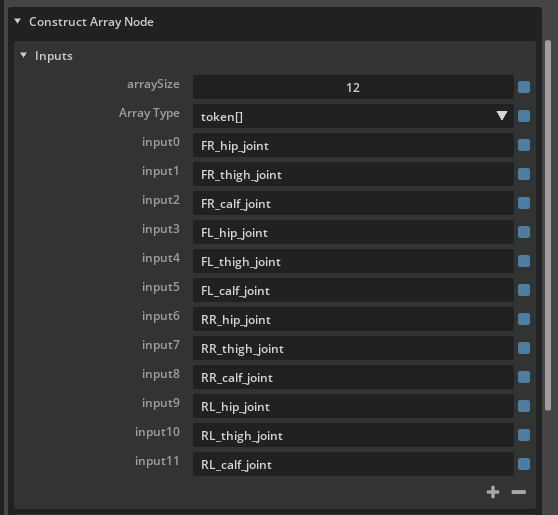
\includegraphics[width=0.5\linewidth]{Zdjęcia/ustawieniaMakeArray.png}
    \caption{Ustawienia bloku Make Array}
    \label{fig:makeArray}
\end{figure}

Blok ROS2Subscriber służy do otrzymywania danych z programu środowiska ROS2, tak zwanego subskrybowania danych, na rysunku \ref{fig:subscriberROS2} pokazano jak poprawnie skonfigurować blok ROS2Subscriber żeby dane były odpowiednio pobierane. Otrzymane dane są przesyłane do bloku Articulation Controller.

\begin{figure}[h]
    \centering
    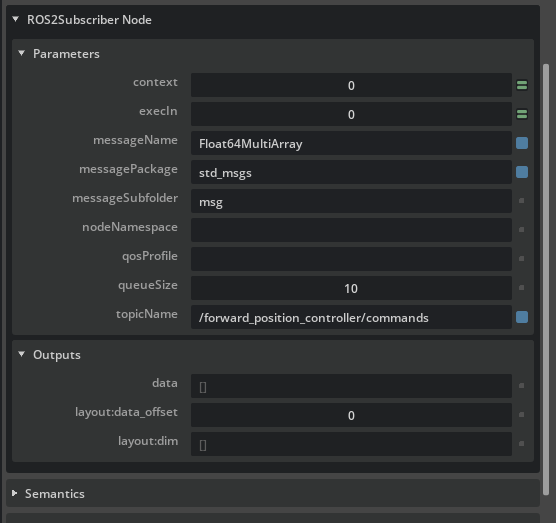
\includegraphics[width=0.5\linewidth]{Zdjęcia/ustawieniaROS2Subsciber.png}
    \caption{Ustawienia bloku ROS2 Subscriber}
    \label{fig:subscriberROS2}
\end{figure}

W celu uruchomienia programu sterującego, po wcześniejszym wypakowaniu potrzebnych plików,  należy przejść do folderu $/quadruped\_robot\_ROS2$ i w terminalu wpisać (żeby uruchomić terminal w danym folderze należy będąc w aplikacji pliki w danym folderze wcisnąć prawy przycisk myszy i ‘otwórz w terminalu’):

$colcon\; build$

Następnie w nowym terminalu wpisać:


$source\; quadruped\_robot\_ROS2/install/setup.bash$

$ros2\; launch robot\_control\; robot\_control.launch.py$

Po czym przechodzi się do folderu $/qudruped\_robot\_ROS2/UI$ uruchamia się nowy terminal w tym folderze i wpisuje:

$python3\; controller.py$

 
Na rysunku \ref{fig:pochyleniePrzod} oraz na rysunku \ref{fig:pochylenieTyl} widoczne jest przykładowe sterowanie cyfrowy bliźniakiem robota Unitree Go2. Sterowanie odbywa się przy pomocy okna z kontrolerem widocznego na obu rysunkach, okno ma nazwę controller.



\begin{figure}[h]
    \centering
    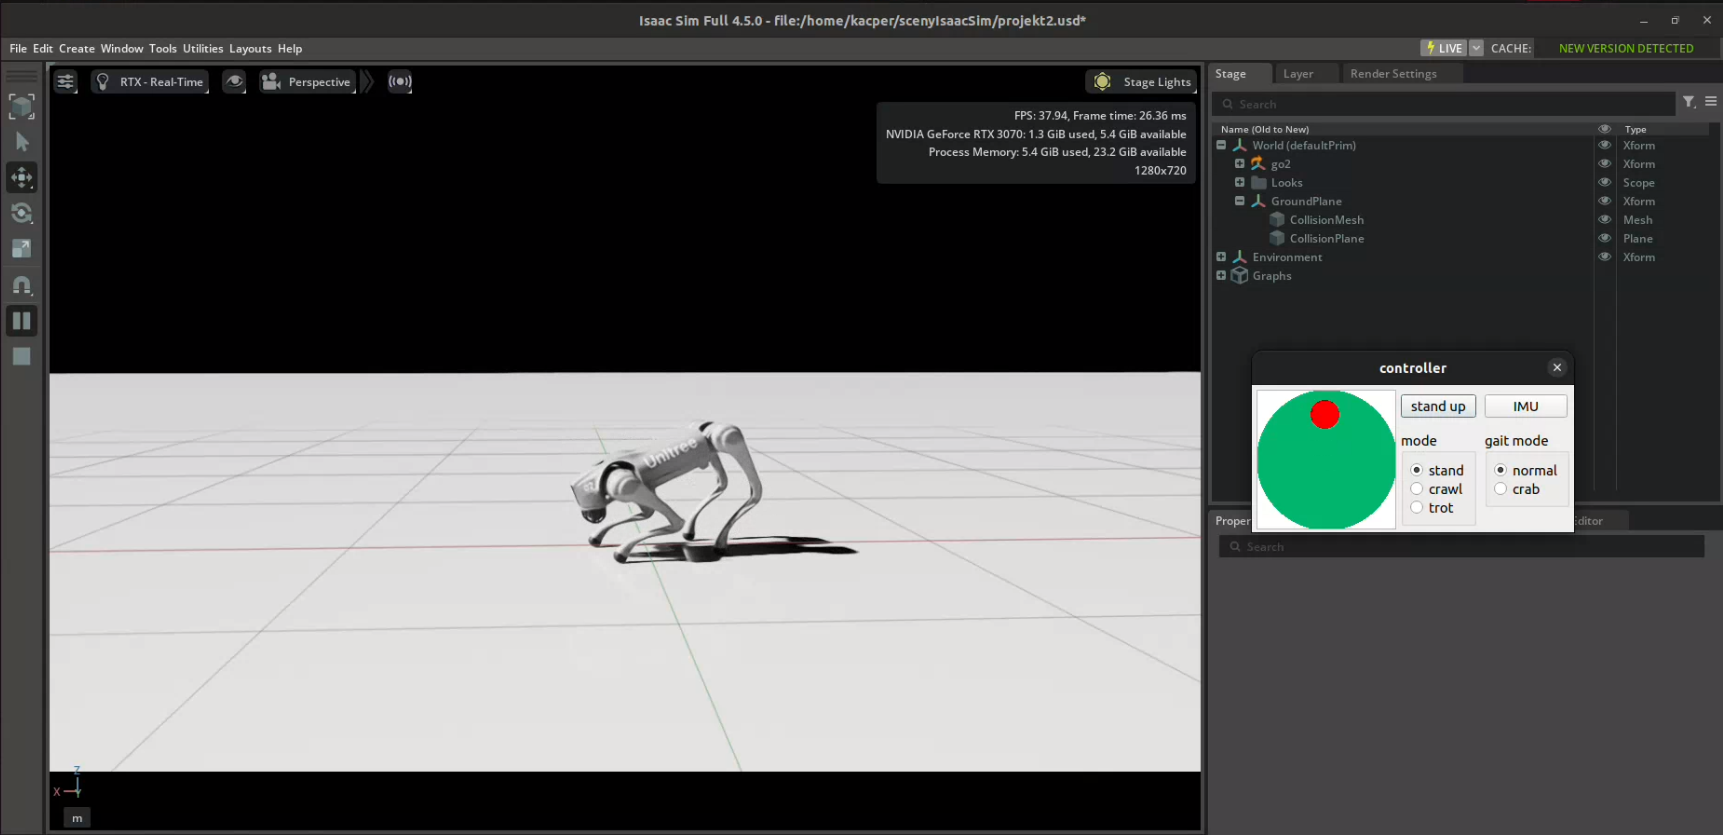
\includegraphics[width=0.75\linewidth]{Zdjęcia/pochyleniePrzod.png}
    \caption{Robot Unitree Go2 pochylający się do przodu.}
    \label{fig:pochyleniePrzod}
\end{figure}

\begin{figure}[h]
    \centering
    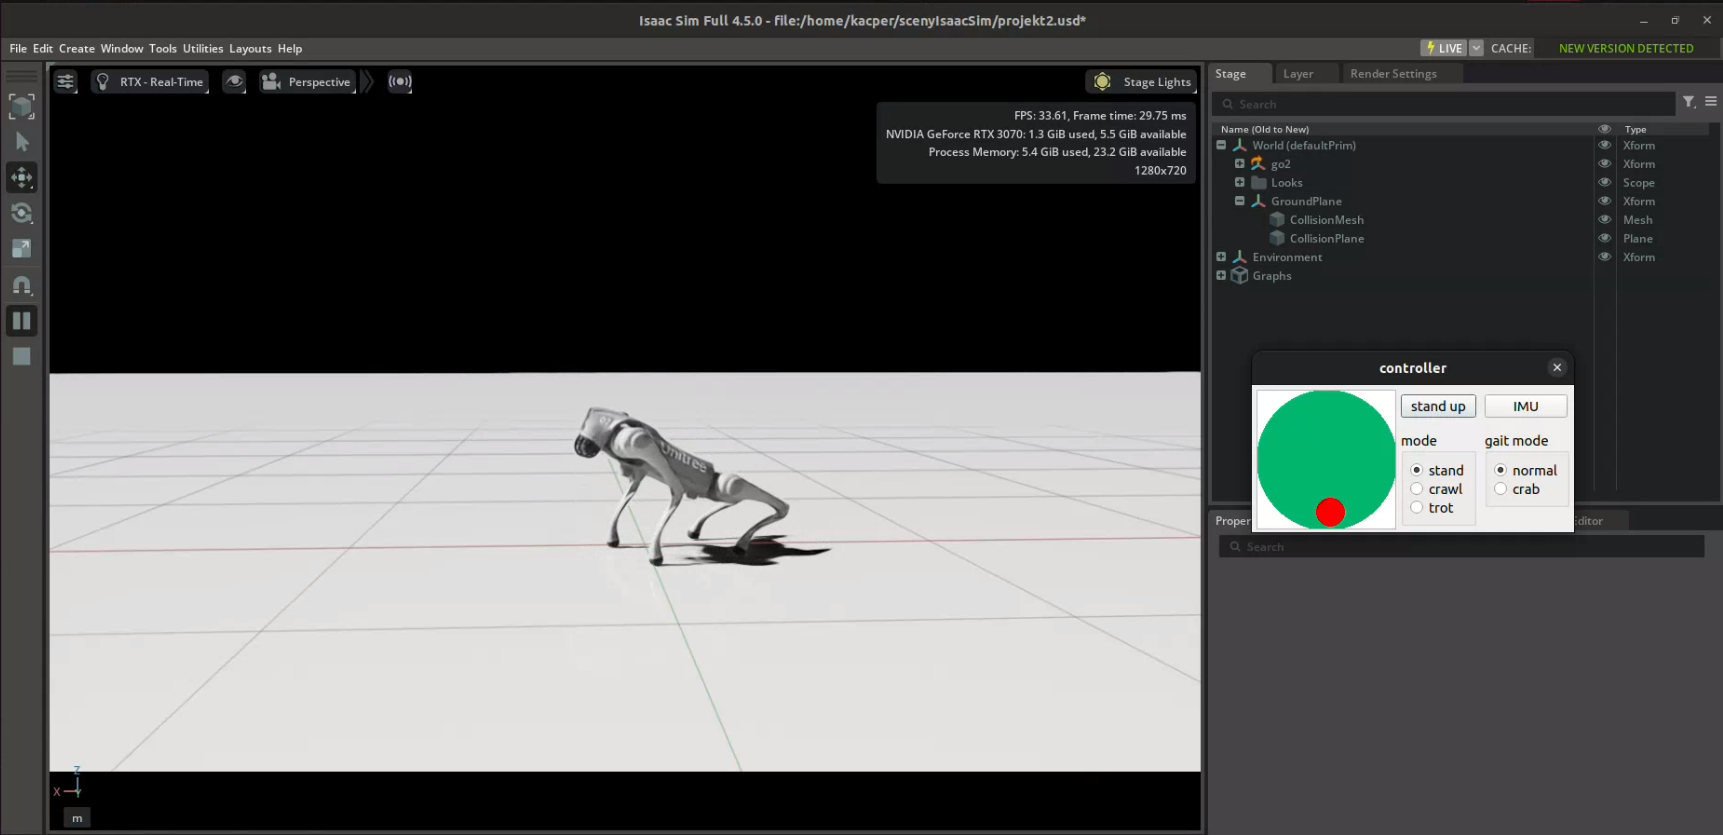
\includegraphics[width=0.75\linewidth]{Zdjęcia/pochylenieTyl.png}
    \caption{Robot Unitree Go2 pochylający się do tyłu.}
    \label{fig:pochylenieTyl}
\end{figure}

Do wykonania tej części projektu korzystaliśmy z poniższego filmu.

\href{https://www.youtube.com/watch?v=L1rpxRm0Q1w&t=581s}{Link do filmu}

\clearpage

\section{Przykładowe symulacje}

W środowisku ISAAC SIM dostępnych jest wiele przykładowych symulacji do, których można uzyskać dostęp, wybierając w górnym pasku Window, następnie Examples, a na końcu Robotics Examples, pokazane jest to na rysunku \ref{fig:symulacje}.
W dolnej części programu otwiera się zakładka Robotics Examples, w której znajdują się różnorodne przykłady umożliwiające sterowanie robotami przy pomocy klawiatury. W dalszej części zaprezentowano wybrane przykłady.



\begin{figure}[h]
    \centering
    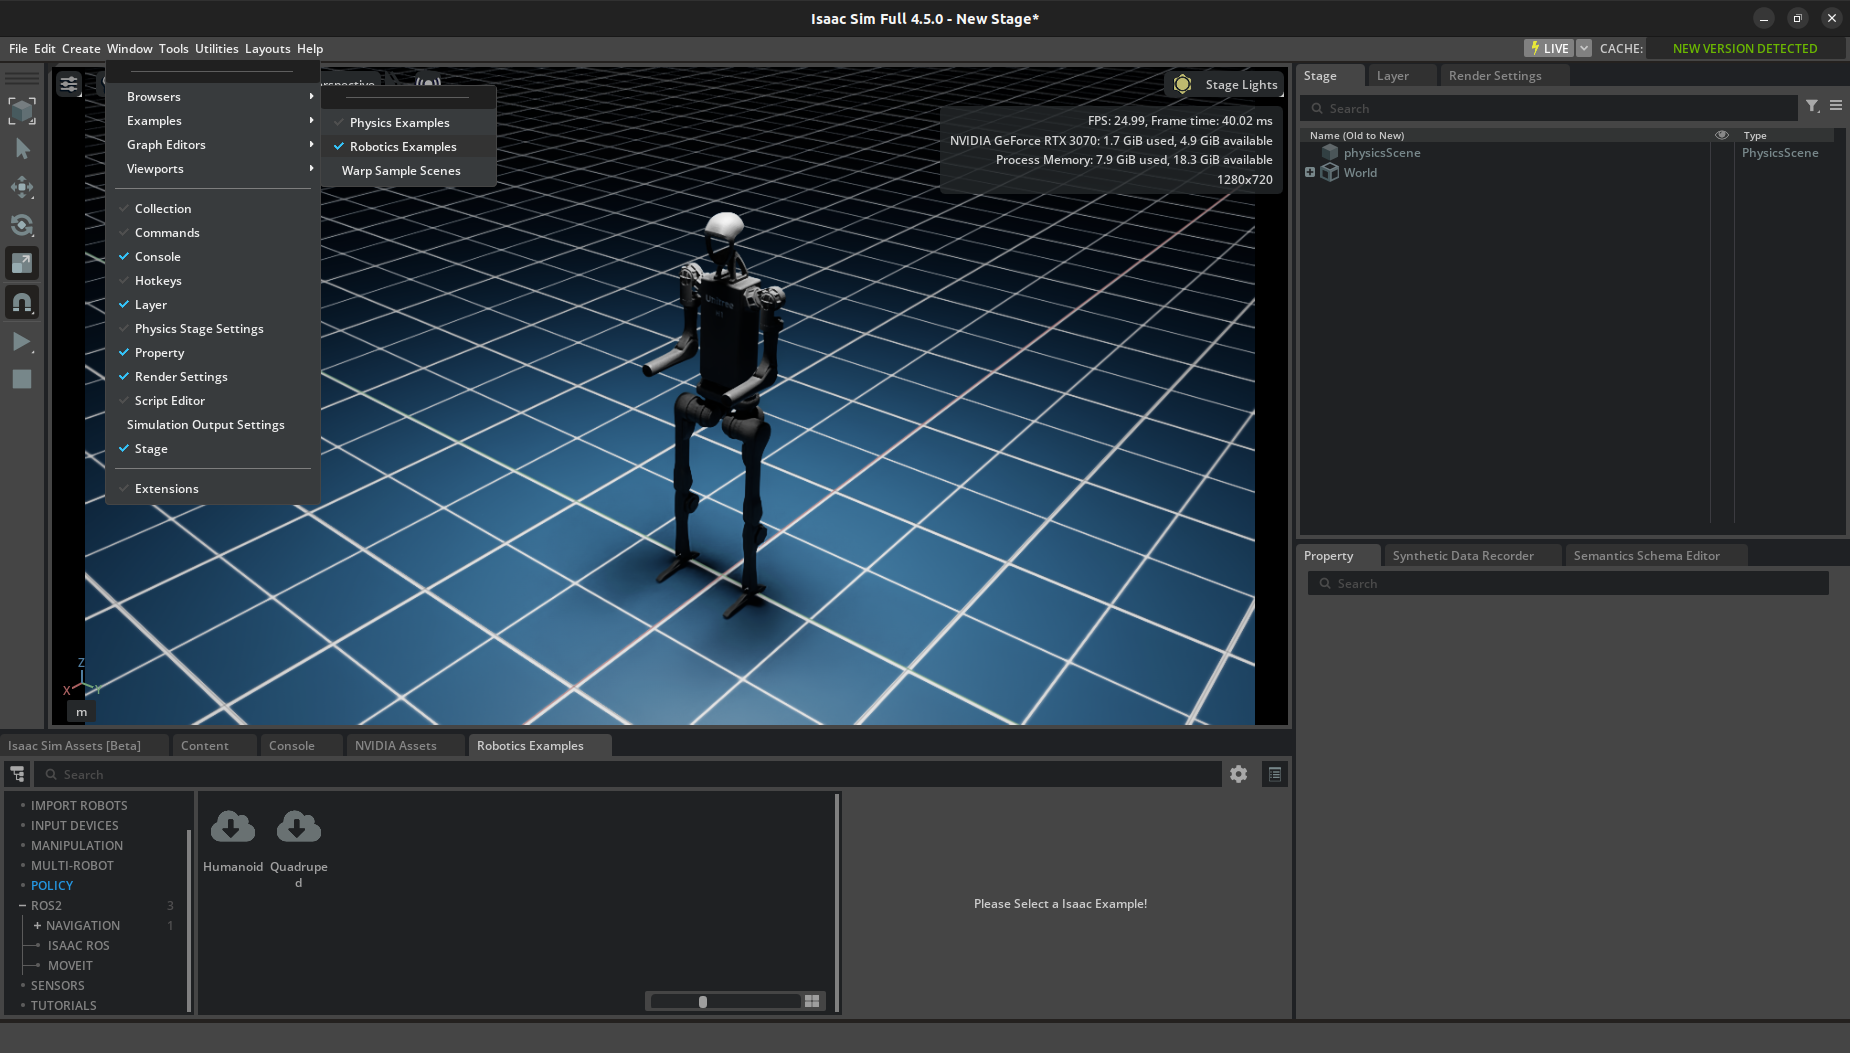
\includegraphics[width=0.5\linewidth]{Zdjęcia/oknoZPrzykladami.png}
    \caption{Okno do dodawania dostępnych w ISAAC SIM przykładowych symulacji.}
    \label{fig:symulacje}
\end{figure}

Na rysunku \ref{fig:bostonDyna} przedstawiony jest widok na cyfrowego bliźniaka firmy Boston Dynamics. W przykładowej symulacji jest możliwe sterowanie nim przy pomocy strzałek i przycisków klawiatury. Podobnie na rysunku \ref{fig:humanoid} pokazany jest humanoidalny robot firmy Unitree nim, również możliwe jest sterowanie w dostępnej przykładowej symulacji.


\begin{figure}[h]
    \centering
    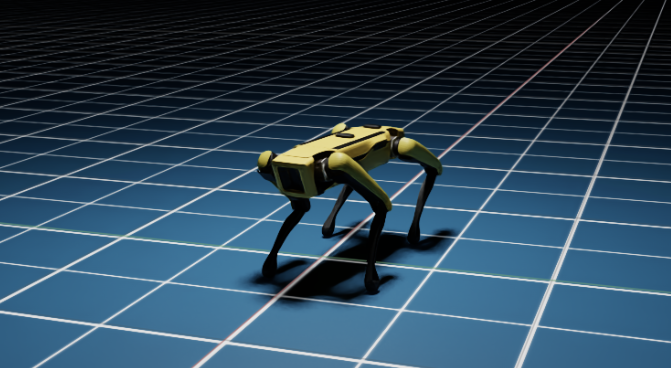
\includegraphics[width=0.5\linewidth]{Zdjęcia/przykladBoston.png}
    \caption{Enter Caption}
    \label{fig:bostonDyna}
\end{figure}

\begin{figure}[h]
    \centering
    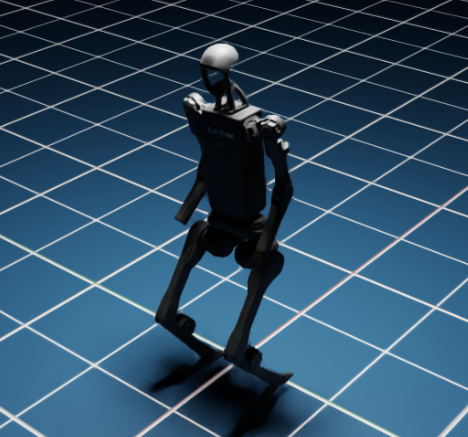
\includegraphics[width=0.5\linewidth]{Zdjęcia/przykladHumanoid.png}
    \caption{Przykład z ISAAC SIM z robotem humanoidalny.}
    \label{fig:humanoid}
\end{figure}

W środowisku ISAAC SIM dostępny jest też przykład z manipulatorem układającym kolejne dostarczane przez ruchomy taśmociąg palety. Okno z widoku tej przykładowej symulacji jest pokazane na rysunku \ref{fig:palety}.

\begin{figure}[h]
    \centering
    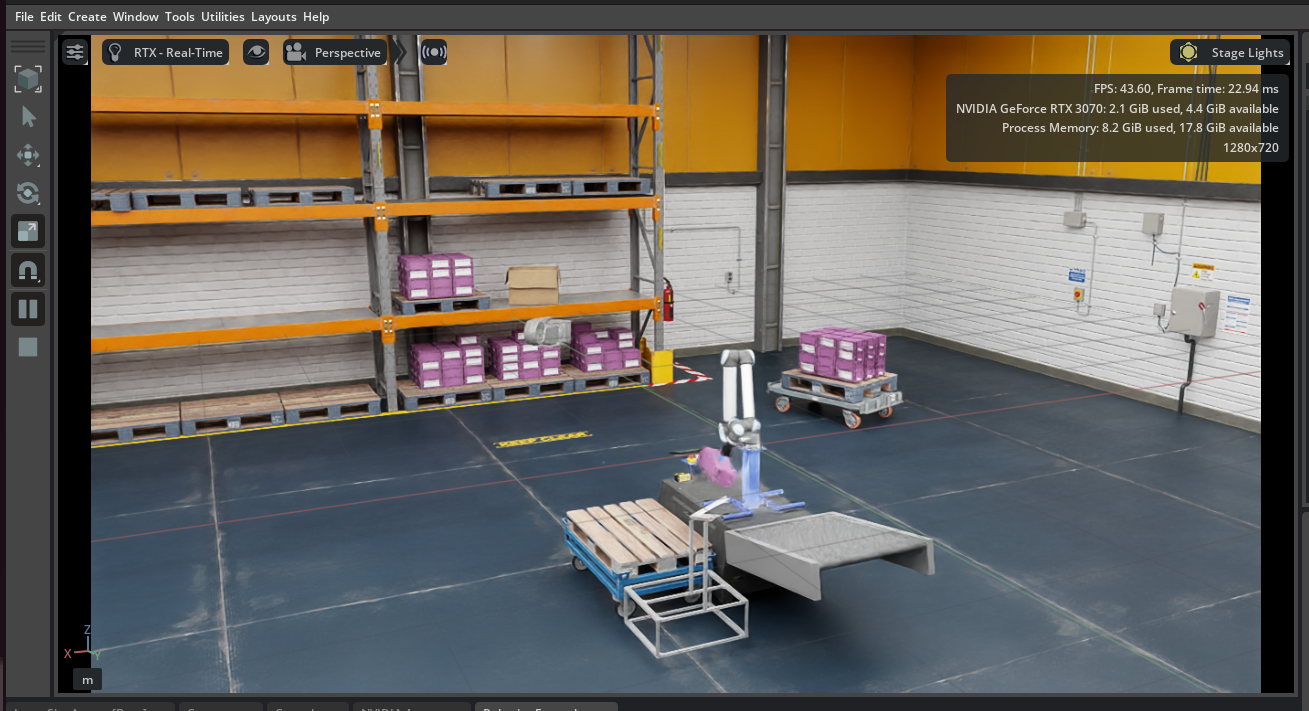
\includegraphics[width=0.5\linewidth]{Zdjęcia/przykladowaPaletyzacja.png}
    \caption{Przykład z ISAAC SIM z manipulatorem i paletami.}
    \label{fig:palety}
\end{figure}

\end{document}
